\subsection{Geïntegreerde aanpak van deadlock}

Het zou beter zijn dat een systeem, i.p.v. 1 strategie te gebruiken, er meerdere kan toepassen, al naargelang de vereiste daartoe.

Zo kan het handig zijn:

\begin{itemize}
\item De bronnen in te delen in een aantal klassen.
\item De strategie ter vermijding van cirkelvormig wachten te gebruiken om deadlock te voorkomen tussen klassen van bronnen te voorkomen.
\item Om per klas een strategie te gebruiken die het best past bij de soorten van bronnen in die klasse
\end{itemize}

 \begin{figure}[htp]
    \centering
            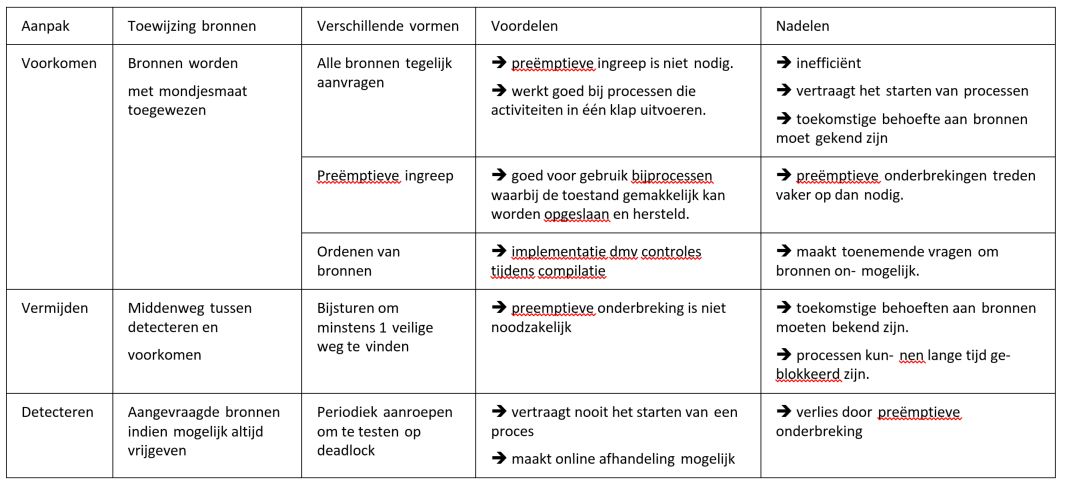
\includegraphics[width=4in]{img/tabelomzettennaartabellatex.PNG}
        \caption{Voorbeeld geen deadlock}
    \label{fig:Voorbeeld geen deadlock}
\end{figure}

